%===
% SUBSECTION: A different approach taken from nuclear physics
%===
\subsec{A recursive expression for phase space integrals}
\label{subsec:recursive-relation}
The problem I ran into at the end of the last section was how to use the energy-momentum delta functions to restrict the bounds of integration. 
I spent some time searching the literature for useful references and the most promising were refs.~\cite{James:1968gu,Byckling:1969sx,Isaacson:2021xty}.
\cite{James:1968gu} provides an introduction to Monte Carlo methods and discusses the phase space measure in sec. 9, which covers several ways to deal with the Dirac delta in the phase space integration measure by doing appropriate changes of variables.
The most useful method, is covered in sec. 9.6 and is the same one used in \cite{Byckling:1969sx}. 
Ref.~\cite{Byckling:1969sx} extends the treatment in sec. 9.6 of~\cite{James:1968gu} by also introducing momentum transfer variables. 
My understanding is that this is appropriate when your matrix element is flat in terms of the momentum transfers.

Consider the phase space integral $R_n(p_a + p_b)$ defined by
\begin{bluenv}{Phase space integral (without $2 \pi$ factors)}
    \vspace{-3ex}
    \begin{equation}
        \label{eq:phase-space-integral-without-2pi}
        R_n(p_a + p_b) = 
        \int \cdots \int \prod_{i=1}^{n} \delta (p_i^2 - m_i^2) \, \Theta(p_i^0) \, 
        \dd^4 p_i \, \delta^4(p_a + p_b - p_1 - \cdots - p_n).
    \end{equation}
    where $p_i$ now denotes a four-momentum vector in constrast to the previous section where it represented a three-momentum magnitude.
    This is manifestly Lorentz invariant and therefore $R_n$ may only be a function of $s \equiv (p_a + p_b)^2$. 
\end{bluenv}


We note that $R_n(s)$ is related to $\dd \Phi_n(s)$ by
\begin{equation}
    R_n(s) = (2\pi)^{3n - 4} \int  \dd \Phi_n(s).
\end{equation} 


Define the new integration variable $M_{n-1}^2 \equiv (p_a + p_b - p_n)^2$. The physical significance of $M_{n-1}$ is that it is the invariant mass of the first $n-1$ particles, which can be seen using four-momentum conservation: $p_a + p_b - p_n = p_1 + p_2 + \cdots + p_{n-1}$.
It is possible to show that the following recursive relation holds (eqn. (3) of \cite{Byckling:1969sx})
\begin{align}
    \label{eq:recursive-phase-space-relation}
    R_n(s) = 
    \int_{(m_1 + m_2 + \cdots + m_{n-1})^2}^{(\sqrt{s} - m_n)^2} 
    \dd M^2_{n-1} \, \int \dd \Omega_n
    \frac{\sqrt{\lambda(s, M_{n-1}^2, m_n^2)}}{8s} R_{n-1}(M_{n-1}^2)
\end{align}
where $\lambda(x, y, z) = x^2 + y^2 + z^2 - 2 xy - 2 xz - 2yz$ and the solid angle $\dd \Omega_n \equiv \dd \cos \theta_n\, \dd \varphi_n$ defines the direction of $\bm{p}_n$ in the frame where $p_a + p_b = (\sqrt{s}, \bm{0})$. 
The upper limit is obtained by requiring that 
\begin{align}
    |\bm{p}_n|^2 = \frac{\lambda(s, M_{n-1}^2, m_n^2)}{4 s}
\end{align}
be positive whereas the lower limit is threshold below which $R_{n-1}(M_{n-1}^2) = 0$.\footnotemark 
 Repeated application of \eref{eq:recursive-phase-space-relation} yields 
\begin{equation}
\begin{aligned}
    R_n&(s) 
        = 
    \int_{(m_1 + m_2 + \cdots + m_{n-1})^2}^{(\sqrt{s} - m_n)^2}
    \dd M^2_{n-1} \,  \int \dd \Omega_n
    \frac{\sqrt{\lambda(s, M_{n-1}^2, m_n^2)}}{8s} \\
        &\times 
    \int_{(m_1 + m_2 + \cdots + m_{n-2})^2}^{(M_{n-1} - m_{n-1})^2}
    \dd M^2_{n-2}  \, \int \dd \Omega_{n-1}
    \frac{\sqrt{\lambda(M_{n-1}^2, M_{n-2}^2, m_{n-1}^2)}}{8M_{n-1}^2} \\
        &\times \cdots \times
    \int_{(m_1 + m_2)^2}^{(M_3 - m_3)^2}
    \dd M^2_{2}  \, \int \dd \Omega_{3}
    \frac{\sqrt{\lambda(M_{3}^2, M_{2}^2, m_{3}^2)}}{8M_{3}^2} 
    \times 
    \int \dd \Omega_2
    \frac{\sqrt{\lambda(M_{2}^2, m_1^2, m_{2}^2)}}{8M_{2}^2}. 
\end{aligned}
\end{equation}
\newpage
The important case for me is when $n = 3$:
\begin{bluenv}{Phase space measure for $n = 3$}
    \vspace{-3ex}
    \begin{equation}
        \label{eq:recursive-LIPS-3}
    \begin{aligned}
        R_3(s) &= (2\pi)^{5}\int \dd \Phi_3(s) \\
            &= 
            \int_{(m_1 + m_2)^2}^{(\sqrt{s} - m_3)^2} \dd M_{2}^2 
            \int \dd \Omega_3 \,
            \frac{\sqrt{\lambda (s, M^2_{2}, m_3^2)}}{8s} \,
            \int \dd \Omega_2 \,
            \frac{\sqrt{\lambda (M^2_2, m_1^2, m_2^2)}}{8 M_2^2} \; .
    \end{aligned}
    \end{equation}
\end{bluenv}
It's easy to verify that the number of integration variables matches our expectation of $3(3) - 4 = 5$ since we are integrating over one invariant mass, and two pairs of two angles. 

In the above discussion we have considered $p_a$ and $p_b$ to be fixed.
However, for my purposes I will also be integrating over $p_a$ and $p_b$.
This case seems to be similar to the one considered in~\cite{Isaacson:2021xty} (cf. the example given between their eqs. (12) and (13)).

\footnotetext{In eq. (3) of~\cite{Byckling:1969sx} the authors allude that the angular $\dd \Omega$ integrals can be performed. They do not perform the integrals because \emph{``the variables defining a momentum vector should appear explicitly if a Monte Carlo method is to be applied for the generation of events.''} In my case I think that we still can't do these integrals trivially because the matrix element depends on them, although I'm not 100\% sure if this is correct.}

\begin{figure}[t]
    \centering
    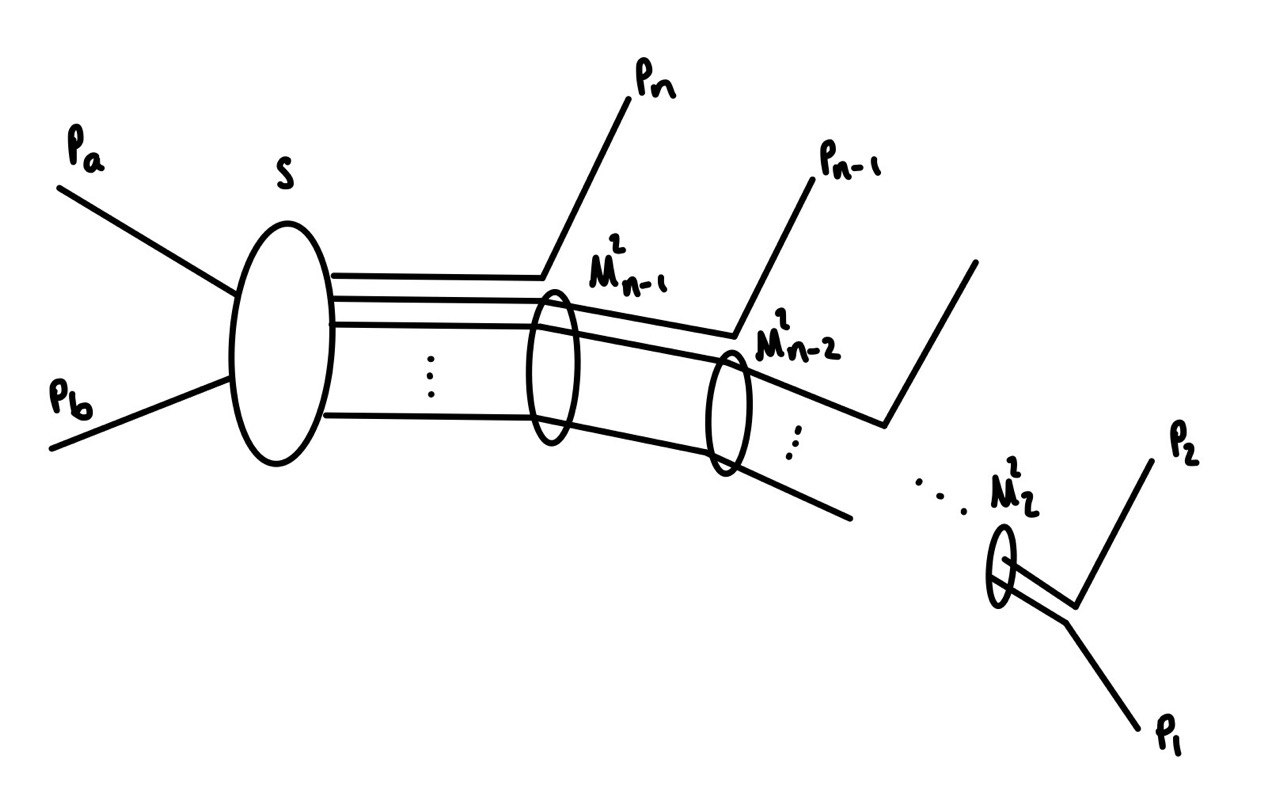
\includegraphics[width=0.6\linewidth]{figs/recursion-diagram.jpg}
    \caption{Illustration of the recursion relation as a sequence of effective $2 \rightarrow 2$ scattering events (this diagram is largely based on pg. 26 of \cite{James:1968gu}).}
    \label{fig:recursion-diagram}
\end{figure}

%====
% SUBSECTION: Writing the integral in terms of momentum transfers 
%====
\subsec{Writing the integral in terms of momentum transfers}
\label{subsec:momentum-transfers}

In sec~\ref{subsec:recursive-relation} we wrote the phase space integral in terms of invariant masses and angles of the three-momenta $\bm{p}_i$ defined in the center-of-mass frame where $\sum_{k=1}^{i} p_k = (M_{i}, \bm{0})$. 
The matrix element in \eref{eq:matrix-element} is a function of the Lorentz invariants $(p_a \cdot p_1), \; (p_b \cdot p_3), \; (p_2 \cdot p_3)$, and $(p_b \cdot p_2) = (- (p_a - p_1 - p_2 - p_3) \cdot p_2)$. 
It is cumbersome to write this matrix element explicitly in terms of the angles $\{ (\theta_i, \varphi_i) : i = 1, 2, \ldots, n\}$ so we would rather use kinematic Lorentz invariants analogous to the Mandelstam variables for $2 \rightarrow 2$ scattering\footnotemark.
To this end it is convenient to \hl{introduce the so-called `momentum transfers' $t_i \equiv Q_i^2 \equiv (p_a - p_1 - \cdots - p_i)^2 = (p_n + p_{n-1} + \cdots + p_{i + 1} - p_b)^2$}.

\footnotetext{At least, I think that is the motivation for introducing these variables.}

Some of the dot products (but not all) may be written exclusively in terms of the kinematic variables. For example,
\begin{gather*}
    \begin{align*}
        t_1 &\equiv (p_a - p_1)^2 &&\rightarrow 
            && 2 p_a \cdot p_1 = m_a^2 +  m_1^2 - t_1 \\
        t_2 &\equiv (p_a - (p_1 + p_2))^2 &&\rightarrow 
            && 2 p_a \cdot p_2 = M_2^2 - m_1^2 + t_1 - t_2 \\
        t_3 &\equiv (p_a - (p_1 + p_2 + p_3))^2 &&\rightarrow 
            && 2 p_a \cdot p_3 = t_2 - t_3 - M_2^2 + M_3^2 \\
        M_2^2 &\equiv (p_1 + p_2)^2 &&\rightarrow 
            && 2 p_1 \cdot p_2 = M_2^2 - m_1^2 - m_2^2 \\
        M_3^2 &\equiv (p_1 + p_2 + p_3)^2 &&\rightarrow 
            && 2 (p_1 + p_2) \cdot p_3 = M_3^2 - M_2^2 - m_3^2 \\
        p_b &= p_1 + p_2 + p_3 - p_a &&\rightarrow
            && 2p_b \cdot p_3 = m_3^2 + t_3 - t_2 \\
        & && && 2p_b \cdot p_2 = 2 p_2 \cdot p_3 + m_2^2 + t_2 - t_1
    \end{align*}
\end{gather*}
I could not write $p_2 \cdot p_3$ in terms of the kinematic invariants alone.
This is because we need $3(3) - 4 = 5$ integration variables. Right now we only have $t_1,\ t_2,\ M_2^2$ which is not enough to fully describe the system; two more are required. 
The additional degrees of freedom are given by the azimuthal angles of the $\bm{Q}_i$ vectors $\varphi_1$, $\varphi_2$ as seen in a frame where $p_a = (m_a, \bm{0})$ (cf. \eref{eq:recursive-momentum-transfer-k} which is eq. (14) of~\cite{Byckling:1969sx}.)
The result for $p_2 \cdot p_3$ in terms of the kinematic invariants $+$ the angles is presented in \appref{app:2-dot-3}.

To transform $R_n$ into a form in which the momentum transfers appear as variables we must consider the phase space integral as a function of $p_a$ and $-p_b \equiv Q_n$ separately: $R_n = R_n(p_a, Q_n)$. 
Let $Q_i = p_a - p_1 - \cdots - p_i$ so that $p_i = Q_{i-1} - Q_i$. 
Then, \eref{eq:phase-space-integral-without-2pi} becomes
\reversemarginpar\marginnote{In \eref{eq:phase-space-integral-with-momentum-transfer} I didn't write the Heaviside function which picks out positive energies, just pretend it is there so that $(Q_{i-1} - Q_i)^0 > 0$.}
\begin{equation}
    \label{eq:phase-space-integral-with-momentum-transfer}
    \begin{aligned}
        R_n(s) 
        &= \int \bigg[
            \prod_{i=1}^{n}
            \dd^4 Q_i \,
            \delta \big( 
                        (Q_{i-1} - Q_i)^2 - m_i^2
                    \big)
            \bigg] \,
            \delta^4 ( p_a + p_b - \sum_{i=1}^{n} (Q_{i - 1} - Q{i})) \vert_{Q_0 \equiv p_a} \\
        &= \int \bigg[
            \prod_{i=1}^{n}
            \dd^4 Q_i
            \delta \big( 
                        (Q_{i-1} - Q_i)^2 - m_i^2
                    \big)
            \bigg] \,
            \delta^4 ( Q_n + p_b) \\
        &= \int 
            \dd^4 Q_{n-1} 
            \delta \big( 
                        (Q_{n-2} - Q_{n-1})^2 - m_{n-1}^2
                    \big) 
            \bigg[
            \prod_{i=1}^{n-2}
            \dd^4 Q_i
            \delta \big( 
                        (Q_{i-1} - Q_i)^2 - m_i^2
                    \big)
            \bigg] \; .
    \end{aligned}
\end{equation}

The recursion relation is then simply
\begin{equation}
    \label{eq:recursion-momentum-transfer}
    R_n(p_a, Q_n) = \int \dd^4 Q_{n-1} \,
        \delta
        \big(
            (Q_{n-1} - Q_n)^2 - m_n^2    
        \big) \, 
        R_{n-1}(p_a, Q_{n-1}) .
\end{equation}
$R_n$ is now regarded as a function of two invariants $s = s_n = (p_a - Q_n)^2$, and $t_n = Q_n^2$: $R_n = R_n(p_a, Q_n) = R_n(s_n, t_n)$. 
Introducing these variables in \eref{eq:recursion-momentum-transfer} the authors of~\cite{Byckling:1969sx} obtain
\begin{equation}
    \label{eq:recursive-momentum-transfer-s-n}
    R_n(s_n, t_n, s_{n-1}, t_{n-1}) = \int \dd s_{n-1} \, \dd t_{n-1} \, 
        K(s_n, t_n, s_{n-1}, t_{n-1}) \, R_{n-1}(s_{n-1}, t_{n-1}) \, ,
\end{equation}
where
\begin{equation}
    \label{eq:recursive-momentum-transfer-k}
    \begin{aligned}
        K&(s_n, t_n, s_{n-1}, t_{n-1}) \\
        & = \int \dd^4 Q_{n-1} \delta(Q^2_{n-1} - t_{n-1}) \, \delta(s_{n-1} - (p_a - Q_{n-1})^2) \, \delta ( (Q_{n-1} - Q_n)^2 - m_n^2) \\
        & = \int_0^{2\pi} \dd \varphi_{n-1} 
            \frac{1}{4 \sqrt{\lambda(s_n, t_n, m_a^2)}} \, 
            \Theta(- G(t_{n-1}, s_n, s_{n-1}, t_n, m_n^2, m_a^2)) \; ,
    \end{aligned}
\end{equation}
$\Theta(x)$ is the Heaviside step-function, and
$\varphi_{n-1}$ defines the azimuthal angle of $\bm{Q}_{n-1}$ in the frame $p_a = (m_a, \bm{0})$. $G$ is a kinematic function defined by
\begin{equation}
    \begin{aligned}
        \label{eq:G-defn}
        G(x,y,z,u,v,w) & = -\frac{1}{2}
        \begin{vmatrix}
            2 u & x + u - v & u + w - y \\
             & 2x & x - z + w \\
            \text{(symm.)} &  & 2w
        \end{vmatrix} \\
        & = x^2 y + xy^2 + z^2 u + v w^2 + v^2 w \\
        & \phantom{=} + xzw + xuv + yzv + yuw \\
        & \phantom{=} - xy(z + u + v + w) - zu (x + y + v + w) - vw(x + y + z + u) \; .
    \end{aligned}
\end{equation}

\begin{bluenv}{$R_n$ for $n = 3$}
    \vspace{-3ex}
    \begin{align}
        R_3(s_3, t_3) 
            = \frac{1}{4\sqrt{\lambda(s_3, t_3, m_a^2)}}
              \int \frac{\dd s_2 \dd t_2 \dd \varphi_2}
                        {4 \sqrt{\lambda(s_2, t_2, m_a^2)}}
              \Theta(- G_2) 
              \int \dd t_1 \dd \varphi_1 \Theta(- G_1)
    \end{align}
    with 
    \begin{gather}
        G_i = G(t_i, s_{i+1}, s_i, t_{i+1}, m_{i+1}^2, m_a^2) \; .
    \end{gather}
\end{bluenv}

To use this method we rewrite the integrand by making the replacements:
\begin{align}
    E_i &\rightarrow \frac{s_{i-1} - s_i - m_i^2}{2\sqrt{s_i}} \\
    2 p_a \cdot p_1 &\rightarrow m_a^2 +  m_1^2 - t_1 \\
    2 p_a \cdot p_2 &\rightarrow s_2 - m_1^2 + t_1 - t_2 \\
    2 p_a \cdot p_3 &\rightarrow t_2 - t_3 - s_2 + s_3 \\
    2 p_1 \cdot p_2 &\rightarrow s_2 - m_1^2 - m_2^2 \\
    2p_b \cdot p_3 &\rightarrow m_3^2 + t_3 - t_2 \\
    2p_b \cdot p_2 &\rightarrow 2 p_2 \cdot p_3 + m_2^2 + t_2 - t_1 \\
    2 p_2 \cdot p_3 &\rightarrow 
        \frac{1}{2 m_a^2} 
        \bigg\{
        % Q1 dot Q2
        \sqrt{\Lambda_1 \Lambda_2}
                - 
                \frac{1}{\sqrt{\lambda_2 \lambda_3}}
                \bigg[
                    m_a^2 \sqrt{G_1 G_2} \cos (\varphi_1 - \varphi_2) \\
                    &\hphantom{=\frac{1}{4 m_a^2}\bigg\{} + 
                    \big(\sqrt{\Lambda_1 \Lambda_2} - 2 (t_1 + t_2 - m_2^2)\big)
                    \big(\sqrt{\Lambda_2 \Lambda_3} - 2 (t_2 + t_3 - m_3^2)\big)
                \bigg] \\
        &\hphantom{=\frac{1}{4 m_a^2}\bigg\{} -
        \bigg(
        % Q1 dot Q3
        \sqrt{\Lambda_1 \Lambda_3} - \sqrt{\frac{\lambda_3}{\lambda_2}} 
                \big[
                    \sqrt{\Lambda_1 \Lambda_2} - 2 m_a^2(t_1 + t_2 - m_2^2)
                \big]
        \bigg)
        \bigg\} \\
        &\hphantom{=}+
        % Q2 dot Q3
        \frac{1}{2}(t_3 - t_2 - m_3^2) \ .
\end{align}

\footnotetext{$M_1^2 = m_1^2$,  $M_3^2 = s$ and  $t_3 = (-p_b)^2 = m_b^2$ are all constants, not integration variables.}  

\newpage
\begin{bluenv}{Random number generation for Monte Carlo}
    To sample $s_i$ we generate a uniform random variable $r_i \sim \mathrm{U}(0,1)$ and compute
    \begin{equation}
        \sqrt{s_i} = r_i \left(\sqrt{s_n} - \sum_{j=1}^{n} m_j\right) + \sum_{j=1}^{n} m_j\ .
    \end{equation}
    Next, we take the generated value of $s_i$ (let's call it $s_i^{\mathrm{gen}}$ and use it to calculate the upper and lower bounds from which we generate $t_i$.
    To do this we solve
    Solve $G(t_{i}, s_{i+1}, s_{i}^\mathrm{gen}, t_{i+1}, m_{i+1}^2, m_a^2) = 0$ for $t_{i}$. 
    This yields,
    \begin{gather}
        \begin{aligned}
            t_{i}^{\pm} 
            =\ 
            &t_{i+1} + m_{i+1}^2 + (2 s_{i+1})^{-1} \\
            & \times
            \bigl[
                (s_{i}^\mathrm{gen} - s_{i+1} - m_{i+1}^2)(t_{i+1} + s_{i+1} - m_a^2) \pm \sqrt{\lambda(s_{i}^\mathrm{gen}, s_{i+1}, m_{i+1}^2)\lambda(t_{i+1},s_{i+1},m_a^2)}
            \bigr] \ .
        \end{aligned} 
    \end{gather}
    So,
    \begin{equation}
        t_i^{\mathrm{gen}} = \gamma_i (t_i^+ - t_i^-) + t_i^-
    \end{equation}
    where $\gamma_i \sim \mathrm{U}(0,1)$ is another uniform random variable. 
\end{bluenv}

